\scanpage{145}
\mspage{19}
Voici les majorations essentielles dans un \unsure{sens|ens.}

\uline{Proposition 3.1} Soit $\pi_0$ le cardinal initial de la filtration cardinale $(\mathrm{Filt}^\pi)_{\pi\ge\pi_0}$ envisagée, $\pi_1$ le plus petit cardinal \inserted{$\ge\pi_0$} tel que les objets de $\mathrm{Filt}^{\pi_0}$ soient $\pi_1$-\,-accessibles,
$C_1=\mathrm{card}\,
\underset{\substack{\Vert\\\underline{\mathrm{Fl}}(M^{\pi_1})}}{
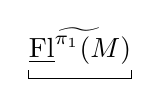
\begin{tikzpicture}[baseline=(F.base)]
\node[inner sep=0pt] (F) {$\widetilde{\underline{\mathrm{Fl}}^{\pi_1}(M)}$};
\draw ([yshift=-2pt]F.south west) -- ++(0,-3pt) -| ([yshift=-2pt]F.south east);
\end{tikzpicture}}{}^*$.
% slanted
\margin{cf plus bas \unsure{la|le} \unsure{notation} $\widetilde C$}

Pour tout cardinal $\pi\ge\pi_0$, je désigne par $M^\pi$ la sous-catégorie \inserted{str.} pleine de $M$ dont l'ens. des objets est $\mathrm{Filt}^\pi$.
\margin{$^*$ \deleted{\unsure{Etant posé}} si $C$ est une catégorie, je désigne par $\widetilde C$ l'ens. des classes d'isomorph. d'objets de $C$. \unsure{Signalons qu'on a toujours} $\mathrm{card}\,\widetilde{\underline{\mathrm{Fl}}(C)}\ge\mathrm{card}\,\deleted{\unsure{\mathrm{Ob}|C}}\widetilde C$ $^*$}
% slanted
\margin{$^*$ Car $\widetilde C\unsure{\hookrightarrow|\leftrightarrow}\widetilde{\mathrm{Fl}(C)}$ via $\unsure{\mathrm{cl}.|\mathrm{cl}}(X)\mapsto\mathrm{cl}(\mathrm{id}_X)$}

1°) Si $r\unsure{\ge|>}\mathrm{Sup}(\deleted{\unsure{\pi_0,}}\pi_{\unsure{1|0}},C_1)$, on a
\[
\mathrm{card}\left(
\underset{\substack{\Vert\\\underline{\mathrm{Fl}}(M^r)}}{
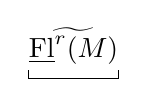
\begin{tikzpicture}[baseline=(F.base)]
\node[inner sep=0pt] (F) {$\widetilde{\underline{\mathrm{Fl}}^r(M)}$};
\draw ([yshift=-2pt]F.south west) -- ++(0,-3pt) -| ([yshift=-2pt]F.south east);
\end{tikzpicture}}
\right)\le 2^{(r^{\pi_0})}
\qquad(=2^r,\text{ si }r=2^c,\text{ avec }c\ge\unsure{r_0|\pi_0}).
\tag*{(3.7)}
\]
2°) Si $r,s\ge\mathrm{Sup}(\pi_1,\deleted{\unsure{\pi_0,}}C_1)$, et si \inserted{$A\in\mathrm{Filt}^r$,} $X\in\mathrm{Filt}^s$, on \unsure{à|a}
\[
\begin{aligned}
\mathrm{Card}\,\widetilde{\underline{\mathrm{Fl}}(M^r_{/X})}
&\le s^{(r^{\pi_0})}\quad
\left\{\begin{aligned}
&=s^r\quad\text{si }r=2^c,\text{ avec }c\ge\pi_0\\
&=s\quad\text{si }s=2^{c'},\text{ avec }c'\ge r^{\pi_0}.
\end{aligned}\right.\\
\inserted{\mathrm{Card}\,\mathrm{Hom}_M(A,X)}&\inserted{\le s^{(r^{\pi_0})}}
\end{aligned}
\tag*{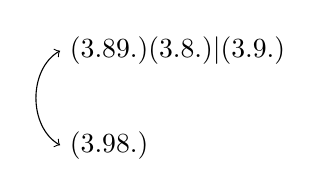
\begin{tikzpicture}[baseline=(a.base)]
\node[anchor=west] (a) at (0,0) {$(3.\deleted{\unsure{8}}9.)\deleted{\unsure{(3.8.)|(3.9.)}}$};
\node[anchor=west] (b) at (0,-1.2) {$(3.\deleted{\unsure{9}}8.)$};
\draw[<->] (a.west) to[bend right=60] (b.west);
\end{tikzpicture}}
\]
\uline{NB} Si on admet l'hypothèse du continu généralisé, qui implique que $\pi^{\pi'}=\pi$ si $\pi>\pi'$ ($\pi$ cardinal infini, $\pi'\ge1$), alors \unsure{pour} \deleted{$r\ge\mathrm{Sup}(\pi_0$} $r$ tel que $r>\pi_0$, les formules précédentes donnent (avec de plus $r\ge\mathrm{Sup}(\pi_1,C_1)$) :
\[
\mathrm{card}\,\widetilde{\underline{\mathrm{Fl}}^r(M)}\le2^r
\tag*{(3.7 bis)}
\]
\[
\begin{aligned}
\mathrm{card}\,\widetilde{\underline{\mathrm{Fl}}(M^r_{/X})}&\le s^r\qquad(\text{si }X\in\mathrm{Filt}^s).\\
\inserted{\mathrm{card}\,\mathrm{Hom}_M(A,X)}&\inserted{\le s^r\quad(\text{si }A\in\mathrm{Filt}^r,\ X\in\mathrm{Filt}^s).}
\end{aligned}
\tag*{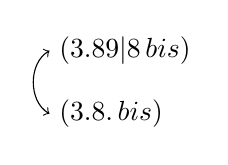
\begin{tikzpicture}[baseline=(a.base)]
\node[anchor=west] (a) at (0,0) {$(3.\deleted{\unsure{8}}\unsure{9|8}\,\text{bis})$};
\node[anchor=west] (b) at (0,-.8) {$(3.8.\,\text{bis})$};
\draw[<->] (a.west) to[bend right=60] (b.west);
\end{tikzpicture}}
\]
Sans hypothèse du continu, ces formules sont \unsure{aussi|encore} valables, pour $r$ de la forme $2^c$, avec $c\ge\unsure{r_0|\pi_0}$.
Ce sont ces \inserted{dernières} formules \deleted{\unsure{qui}} ont l'air les plus naturelles. Pour (3.8. bis), \inserted{et (3.9. bis)} je \unsure{signale|rappelle} que le $2^e$ membre $s^r$ est le cardinal de l'ens. $\mathrm{Hom}_{\mathrm{Ens}}(A,X)$, si \deleted{$\unsure{A|A_2}$} \inserted{$A,X$ sont deux ens. tels que} ($\mathrm{card}\,A=r$, $\mathrm{card}\,X=s$. On ne peut donc espérer améliorer (3.8 bis)! Pour le
% archive sheet number: 144
